A wide variety of attacks can be posed against a system like this; there are web components, arbitrary code executions and legitimate cross-domain requests that may be abused. Therefore, it is crucial to discuss the topics at length and disclose what strengths and weaknesess are present from the get-go.

\subsection{Authentication}
Authentication for the frontend is managed using an authentication interceptor. The main purpose of this device is to modify all requests by setting the authentication field in the header of the request for authenticated users. It also collects failed requests in the case of token expiration and tries to refresh the token to retry all failed requests automatically and stay logged in without the user being aware of affected.
\begin{sidewaysfigure}
    \centering
    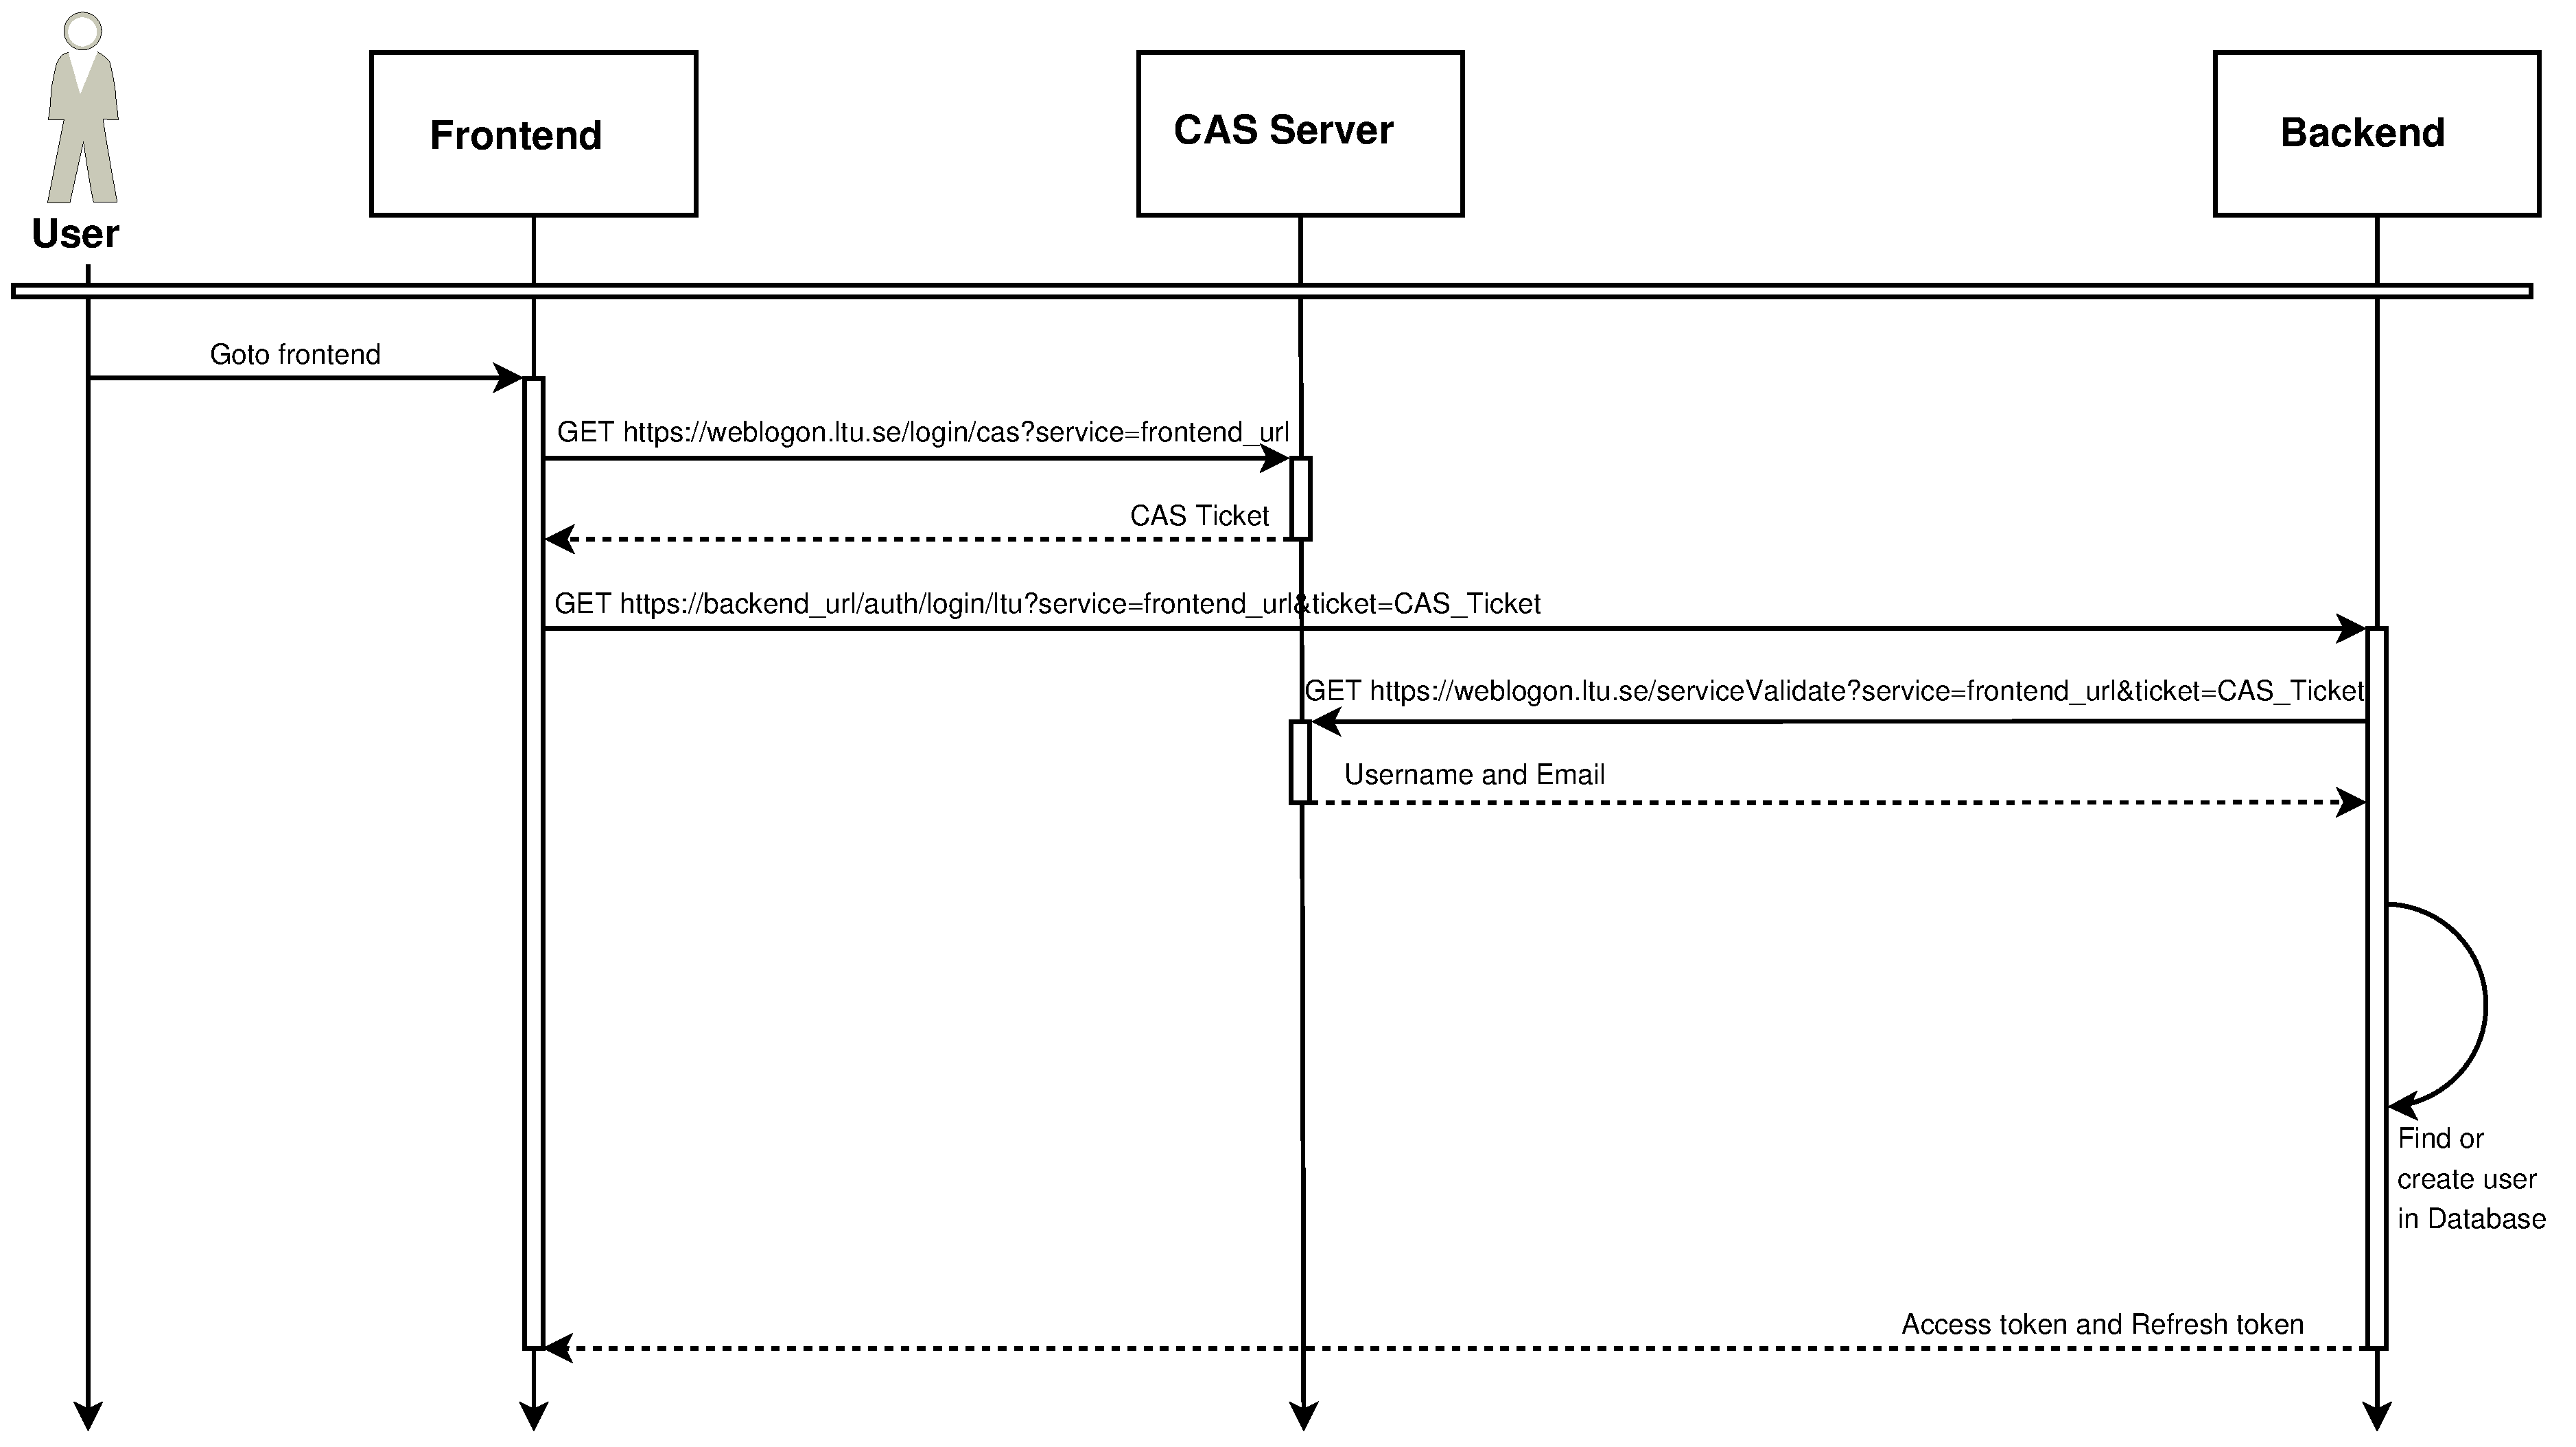
\includegraphics[width=\textwidth]{img/authentication_sequence.eps}
    \caption{Successful authentication sequence.}
    \label{fig:auth}
\end{sidewaysfigure}

%\subsubsection{Authentication}
The API endpoint \url{/auth/login/ltu} validates a service ticket issued by CAS at \url{https://weblogon.ltu.se/cas/login} and, if successful, will issue an access token for use at the other access restricted endpoints of the API (see figure~\ref{fig:auth}). The access token is a JSON Web Token with a short life span, that is tamper-proof and contains information about the user's id and access level. This approach allows the backend to remain sessionless, as the backend will validate the token at every API request. Since the access token expires quickly a refresh token is issued alongside it. The refresh token has a much longer life span and its only use is to generate new access tokens at the \url{/auth/login/accesstoken} endpoint. The refresh tokens are stored in the database, while the access tokens are not. Revoking a refresh token is done by deleting it from the database. Theft of an access token or refresh token would give the thief access until the token expires or, in the case of refresh tokens, until it is revoked. Stealing tokens is made harder with SSL encryption.

Currently logging in with CAS via \LTU\ is the only way to access the backend. This could however be extended to allow more ways of logging in by adding other authentication endpoints to the backend.

\subsection{HTTPS} \label{https}
Self-signed certificates were used for the testing environment in order to establish a secure environment with HTTPS. Once a proper production environment is used, it is necessary to use a trusted certificate authority instead of self-signed certificates.

\subsection{Input Validation}
Injection attacks are a common security problem in applications that use databases. To prevent this the API has to make sure the input has the expected form. A boolean input field must be of boolean type to be accepted. To achieve this, the module \href{https://github.com/ctavan/express-validator}{express-validator} was used. With this module it's possible to check URL, query and body input. For every invalid input field a specific error message is added to an array. When all fields have been checked, this array will be returned together with an HTTP error code \texttt{400:\@ Bad Request} as feedback. This way the user can receive direct feedback without the need to consult the documentation.

% SSL (HTTPS), just mention it
\subsection{Access Control}
The API has three different base roles:
\begin{itemize}
\item Basic
\item Advanced
\item Admin
\end{itemize}
These are assigned according to the user's role in their school, which is found when logging in through CAS. If the user is a student, a basic role will be assigned, and if the user is a teacher, an advanced role will be assigned. Admin is never assigned automatically and has to be set manually if needed. Depending on the role, different limitations are enforced. A basic user is only allowed to create 3 courses. Admins and advanced users are allowed to create an unlimited number of courses. This is currently the only difference between a basic and an advanced user. The reason a basic user is limited in their number of courses is simply to prevent malicious behaviour. Admins have full access to every route and are not limited in any way. This is mostly affecting course routes.

Regardless of a user's base role he has a different role in every course. Every course in turn has three user roles:
\begin{itemize}
\item Student
\item Teacher
\item Owner
\end{itemize}
Students are only allowed to use a subset of the routes, such as submitting assignments or leaving courses. The teacher role maintains the course, but also controls who is allowed to join. The highest course role is the owner, which is the user that created the course. The owner can do everything a teacher is able to do, the only difference being that teachers can't remove the owner from the course. A user with the admin base role is basically able to do everything in any course.

\subsection{Tester Sandbox}
Arbitrary code execution is as dangerous as it sounds and needs to be handled accordingly. The approach taken here is to sandbox the environment using containers and to simply trust the container software maintainers to fix whatever vulnerabilities arise.

After each series of tests, the container is considered ``spent''. That is, no series of tests may influence any other of series of test, and should the code, for instance, rewrite the programming environment, it will not influence the later tests.

\subsection{Remote Attacks}% Using Tester}
While sandboxing resolves issues regarding result correctness, it does not relieve the administrator from the responsibility of denying attempts at remote attacks from ephemeral tester shells. One could picture a scenario (see figure~\ref{fig:tester-ddos}) where tester-clusters are used to amplify attacks made from zombie shells by supplying as many parallel malicious scripts as the tester environment will allow.
\begin{figure}[ht]
    \centering
    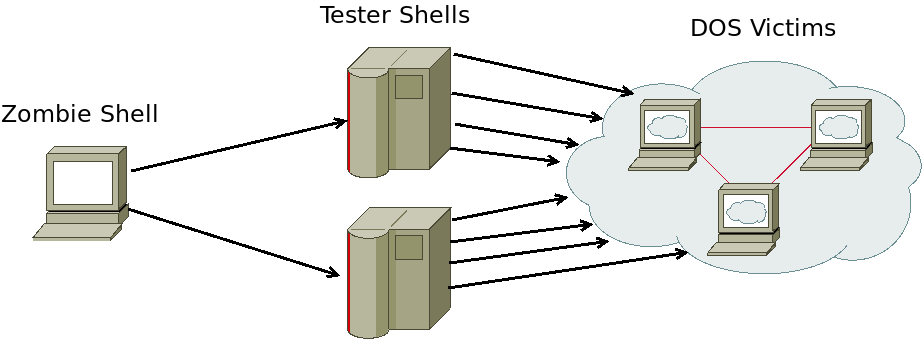
\includegraphics[width=\textwidth]{img/tester_amplification.png}
    \caption{A DDOS scenario involving unsecured tester environments.}\label{fig:tester-ddos}
\end{figure}
If the tester shells are allowed to access the network, an adversary could send test-requests to backends (or public testers) that would in turn make requests to remote hosts. This could partly act as a proxy for some attacker that would like to remain anonymous, but also allow one remotely controlled host to attack many other hosts.

There are multiple ways to solve this security concern and they all come with their own drawbacks and advantages. Firstly, there is the option to simply allow connections to be made, but implement a rate limit to keep malicious use down. This takes away the risk of a distributed denial-of-service (DDOS) scenario, where testers could be exploited to deliver large amounts of illicit traffic. However, it would require tester to keep track of which users are allowed to use the network.

Secondly, there is the option to block all communications but the one made to the runner itself. By doing so, the attack vector is minimized and unlikely to cause any trouble. Unfortunately, that would also remove the ability to create assignments that connect to the web for some information, such as scraping exercises. Furthermore, it would require careful setup of firewall rules within the runner that should not be possible to manipulate by the user running the test.

Lastly, much like the second suggestion, there is the option to allow outgoing connections, but place the tester behind NAT (Network Address Translation). Then, firewall rules can be placed on the network to allow/deny connections based on origin and context. This is simpler than the second option, but lets containers hosted under the same NAT contact one another. This means that sending recursive testing requests may be possible.

In order to avoid making the solution needlessly complex, the last method was decided upon. Since \docker{} provides a virtual network mode to place its containers behind NAT, no additional work had to be done in order to set the protection up. Furthermore, the risk of having malicious users perform recursive tests leading to denial of service was deemed small in the context of the development environment.

\subsection{Dumping Assignments}\label{sec:dumping}
During development, it was found that on some setups, assignments could be dumped with relative ease from memory using standard GNU utilities and code input from the frontend interface. An interesting aspect to note is that since containers share kernel, the protection that usually wards unauthorized users from reading other users' memory varied between kernel versions.

For instance, some payload \texttt{dump.py} would happily extract the memory of the part of tester that ran on docker and executed the python files. This memory in turn contained the answers to the tests that a student would need to complete, effectively allowing a constant-time lookup table to be constructed.

When run on a Debian GNU/Linux host, the exploit worked flawlessly, whereas the same script on an Arch Linux host would deny access and halt. This lead to the decision of running all user-supplied code as a non-root user, which seems to have taken care of the bulk of such memory-access vulnerabilities.

\subsection{Hijacking TCP Sessions}
Another vulnerability that was identified was the ability to hijack the TCP sessions used to transport test results. The authors acknowledge that an attack like this probably still affects the system, but decided that it is too far out of scope for them to fix.
\begin{wrapfigure}[10]{l}{7cm}
    \centering
    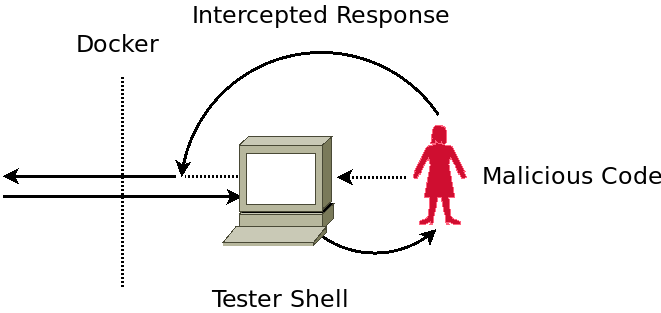
\includegraphics[width=.35\textwidth]{tcp_interception.png}
    \caption{A TCP hijack may send data pretending to be the tester.}
\end{wrapfigure}

In fact, should an enterprising student attempt to trick the system by performing such an attack, they should be rewarded for their investigative work, rather than punished for gaming the system. By triggering such a response, the student has clearly shown that they aspire for more than a simple grade and probably do not require gamification to go further.
